\documentclass[11pt,a4paper]{article}
\usepackage[T1]{fontenc}
\usepackage{lmodern}
\usepackage[utf8]{inputenc}
\usepackage{amsmath,amssymb,amsthm}
\usepackage{booktabs}
\usepackage{graphicx}
\usepackage{microtype}
\usepackage[margin=2.6cm]{geometry}
\usepackage[hidelinks]{hyperref}
\usepackage{natbib}

\newtheorem{lemma}{Lemma}
\newtheorem{proposition}{Proposition}
\theoremstyle{definition}
\newtheorem{definition}{Definition}

\title{\bfseries How Many Independent Models Does an Open-Model\\
Ecosystem Contain? Evidence at the Exact Conditional Null}

\author{Shaurya Gupta\\\small\texttt{shauryaguptaa8@gmail.com}}
\date{\today}

\begin{document}
\maketitle

\begin{abstract}
\noindent
Whether independently developed language models fail on the same inputs bears directly on
systemic risk, ensemble reliability, and model-as-judge evaluation. Recent work has shown that
the answer depends on the null model chosen, and concluded that monoculture inference is
therefore \emph{subjective}, leaving open which null is appropriate
\citep{jo2026subjectivity}. We argue that one null is canonical rather than arbitrary. Because
the row and column margins of a model-by-item outcome matrix are the jointly sufficient
statistics of the Rasch family, the uniform distribution over margin-matched matrices is the
unique \emph{exact, fit-free} conditional null for that entire family: it estimates no
parameters, applies no penalty, and makes no identification choice. We report what the answer
is at that null, on $1{,}228$--$1{,}373$ open models per benchmark across five benchmarks --- a
population three times larger than previously analysed.

At the mean level there is nothing to find, and this is a theorem rather than a measurement:
mean pairwise co-failure is a function of the item margins alone, so its excess over any
margin-preserving null is identically zero. We show this degeneracy has been proved
independently in three literatures --- as Schluter's V-ratio in ecology, as Kuder--Richardson /
Cronbach's $\alpha$ in psychometrics, and as Fleiss's observed agreement for the multi-category
case --- and give the translation between them, since none is cited in the model-evaluation
literature. Empirically the measured excess matches the closed form to $10^{-16}$ on all five
benchmarks. Our pre-registered dispersion statistic came out \emph{below} its null on three of
five benchmarks and above on two; its pre-registered kill condition fired and we report it as
refuted.

What survives is second-order and large. Conditioning on the margins leaves residual correlation
with root-mean-square $0.248$ against $0.039$ under the exact null --- a sixfold excess --- and
five eigenvalues above the null spectral edge. We deliberately do \emph{not} report this as an
``effective number of independent models'': we show that the participation ratio is
algebraically $N/(1+(N-1)\overline{R_{ij}^2})$, so it cannot distinguish one weak global factor
from many tight clusters, and we give the diagnostics that can. Misspecification controls show
that two-parameter discrimination heterogeneity cannot generate the observed effect
(rms $\le0.076$), but a low-dimensional multi-ability structure generates much of it
(rms $0.162$); the observed spectral signature resembles the latter, not duplicated model
families. The honest reading is therefore that open-model failure is governed by a handful of
latent dimensions beyond unidimensional ability. We also reconcile two apparently contradictory
statistics exactly --- the excess variance is $29\times$ the null while its covariance with the
margin-model prediction is strongly negative --- and show the effect is not an artifact of
duplicate models, chain mixing, or the choice of spectral functional. A pre-registered test on
real model responses (not just correctness) finds that our own critique does \emph{not} rescue
one specific published claim: the reported association between model accuracy and error
agreement attenuates only $12\%$ under conditioning and remains significant, so that finding is
reported as robust rather than reinterpreted.
\end{abstract}

\section{Introduction}

If many deployed models share blind spots, diversification is illusory: an ensemble, a panel of
model judges, or a market of competing screening vendors supplies far less independent evidence
than its headcount suggests. A growing literature measures how often models err together, and
almost all of it shares one pattern: record which models fail which items, then compare the
rate at which pairs fail together against a baseline in which they are assumed independent.

\citet{jo2026subjectivity} showed that this comparison is highly sensitive to the assumed
baseline --- conditioning on item difficulty leaves residual correlations ``substantially
attenuated'', with ``some even flipping from strongly positive to slightly negative'' --- and
proved that a sufficiently expressive null can explain away any observed dependence. Their
conclusion is that monoculture is a context-dependent inference problem, and they state
explicitly that their framework ``does not prescribe which null is right''.

We take up that open question. Our claim is that the ladder of nulls has a canonical rung. The
row and column margins of a binary outcome matrix are the jointly sufficient statistics of the
Rasch model; conditioning on them therefore removes the entire nuisance family without
estimating any of it. The resulting null --- the uniform distribution over margin-matched
matrices, known in ecology as the fixed-fixed null and in psychometrics as the Rasch conditional
null --- requires no gradient ascent, no regularisation, and no identification convention. It is
the point at which ``we conditioned on ability and difficulty'' stops being an analyst's choice
and becomes an exact statement.

\paragraph{Contributions.}
\begin{enumerate}
\item \textbf{A canonical stopping point.} We identify the exact conditional null implied by
Rasch sufficiency as the non-subjective answer to the null-selection problem posed by
\citet{jo2026subjectivity}, and report what the answer is there
(Section~\ref{sec:canonical}).
\item \textbf{A translation table across three literatures.} The degeneracy of mean co-failure
under margin-preserving nulls is Schluter's V-ratio result in ecology
\citep{schluter1984,gotelli2000,gotelliulrich2012}, Kuder--Richardson/Cronbach's $\alpha$ in
psychometrics \citep{kuder1937,cronbach1951}, and Fleiss's observed agreement in the
multi-category case \citep{fleiss1971}. None is cited in the model-evaluation literature. We
state the identities and attribute them (Section~\ref{sec:degeneracy}).
\item \textbf{A calibrated measurement of residual structure at scale}, over
$1{,}228$--$1{,}373$ models per benchmark, together with a negative result about the statistic
most tempting to report: the participation ratio is a monotone transform of mean squared
residual correlation and does not count independent models (Section~\ref{sec:results}).
\item \textbf{An exact reconciliation of two contradictory-looking results}, and robustness to
deduplication, mixing, and functional choice (Sections~\ref{sec:reconcile}--\ref{sec:robust}).
\item \textbf{A released substrate and estimator}, harvested at zero inference cost, with the
harness pitfalls documented (Section~\ref{sec:data}).
\end{enumerate}

\paragraph{What we do not claim.} We do not claim prior measurements were computed incorrectly,
nor that language models are in fact diverse. We claim that a class of baseline cannot separate
shared behaviour from shared item difficulty; that a canonical baseline exists; and that at that
baseline the concentration conclusion survives in a different and more defensible form than the
one usually reported.

\section{Setup}

Let $F\in\{0,1\}^{N\times M}$, $F_{im}=1$ iff model $i$ fails item $m$. Write $r_i=\sum_m F_{im}$,
$c_m=\sum_i F_{im}$, $p_i=r_i/M$, $f_m=c_m/N$, $\bar f=\frac1M\sum_m f_m$, and
$C_{ij}=\frac1M\sum_m F_{im}F_{jm}$.

\section{The mean is degenerate, and this is known}
\label{sec:degeneracy}

\begin{lemma}[Mean co-failure depends only on item margins]
\label{lem:mean}
$\displaystyle O \;=\; \frac{1}{M N(N-1)}\sum_{m}\bigl(c_m^{2}-c_m\bigr).$
\end{lemma}

\begin{proof}
$\sum_{i\neq j}F_{im}F_{jm}=(\sum_i F_{im})^2-\sum_i F_{im}^2=c_m^2-c_m$ since $F_{im}\in\{0,1\}$.
\end{proof}

Consequently any randomisation preserving the column margins leaves $O$ invariant with zero
variance, and the standardised effect size for $O$ is $0/0$.

\paragraph{This is not new, in three separate fields.} In ecology it is the degeneracy of
Schluter's V-ratio \citep{schluter1984}. \citet{gotelli2000} states plainly that ``the V ratio
was not used in this analysis because retaining row and column totals as in SIM9 does not ever
change the index'', and \citet{gotelliulrich2012} generalise the warning to the S\o rensen,
Simpson, Morisita and NODF families. In psychometrics the same content appears as reliability:

\begin{lemma}[The independence-baseline excess is reliability times difficulty variance]
\label{lem:alpha}
With $I$ the mean of $p_ip_j$ over ordered pairs,
\[
O-I=\frac{N\operatorname{Var}_m(f_m)+\operatorname{Var}_i(p_i)-\bar f(1-\bar f)}{N-1}
   \;=\;\alpha_N\cdot\operatorname{Var}_m(f_m),
\]
where $\alpha_N$ is Cronbach's $\alpha$ computed with the $N$ models in the item role
\citep{kuder1937,cronbach1951}.
\end{lemma}

\noindent We verified the second equality numerically: residual $\le 6.9\times10^{-17}$ across
five shapes with $N\in[25,1200]$, $M\in[45,900]$, and $-4.2\times10^{-17}$ on the real ARC
matrix, where $\alpha_N=0.99928$. Since $\alpha_N\to1$ for large $N$, the reported ``excess
co-failure'' is, to an excellent approximation, simply the cross-item variance in difficulty ---
strictly positive whenever items differ in difficulty, including when every model fails
independently. The asymptotic statement is the de Finetti / beta-binomial identity, and
\citet{yule1903} is the classical warning about association induced by mixing.

For multi-category responses the analogous statistic --- the rate at which two models give the
same wrong answer given both are wrong, as used by \citet{kim2025correlated} against a uniform
$1/(K-1)$ baseline --- is Fleiss's observed agreement \citep{fleiss1971},
$\sum_m\sum_k n_{mk}(n_{mk}-1)/\sum_m n_m(n_m-1)$, and depends on the per-item response
composition alone. In a simulation where models err \emph{conditionally independently} given the
item, drawing from a shared per-item distractor-attractiveness distribution, we observe agreement
$0.5567$ against a uniform baseline of $0.3333$ --- an apparent excess of $+0.2233$ --- while the
excess over the composition-preserving null is $-1.1\times10^{-16}$. This is the founding premise
of answer-copying detection \citep{wollack1997,vanderlinden2006}, and we restate it rather than
claim it.

\paragraph{Why restate known results.} Because the model-evaluation literature cites none of
them, and because the three statements are the same theorem in three notations. Making the
bridge explicit is the cheapest available correction to a measurement practice now in active use.

\section{The canonical null}
\label{sec:canonical}

\citet{jo2026subjectivity} prove that any distribution on $\{0,1\}^m$ is a mixture of
conditionally independent Bernoullis, so excess dependence shrinks monotonically as the null
grows more expressive; they conclude the choice is subjective. We observe that the ladder has a
distinguished rung.

The Rasch model $\Pr(F_{im}=1)=\sigma(\alpha_i+\beta_m)$ has $\{r_i\}$ and $\{c_m\}$ as jointly
sufficient statistics. Conditioning on both therefore eliminates $\alpha$ and $\beta$ exactly,
and the conditional law of $F$ given its margins is \emph{uniform} on the set of margin-matched
binary matrices, for every parameter value \citep{rasch1960,andersen1973}. That set is precisely
the ecologists' fixed-fixed null, sampled here with curveball \citep{strona2014}; the
equivalence between the two traditions is standard
\citep{besag1989,ponocny2001,verhelst2008,miller2013}.

The practical consequence is that this null estimates nothing. A fitted IRT null requires a
parameterisation, an optimiser, penalties, and an identification convention, each of which is a
defensible-but-arbitrary analyst choice of exactly the kind \citet{jo2026subjectivity} identify.
The conditional null has none. It is the strongest ability-and-difficulty control that can be
applied without fitting, and it is unique in that respect.

\paragraph{Margin-conditioned excess.} For a point estimate of the null mean we use the
maximum-entropy (Rasch) mean field $P_{im}=\sigma(\alpha_i+\beta_m)$, fitted to a maximum
absolute margin error of $5.7\times10^{-13}$, and
\[
D \;=\; \frac{FF^{\!\top}-PP^{\!\top}}{M}.
\]
The mean field is validated against the randomisation itself: over $319{,}600$ model pairs the
curveball expectation of $C_{ij}$ and the Rasch prediction correlate at $0.99999$, mean absolute
difference $0.00039$ on a level of $0.2849$. The matrix $D$ is the excess matrix of the
network-backbone literature \citep{neal2021}.

\begin{definition}[Effective number of independent models]
Let $R$ be $D$ scaled to unit diagonal, with eigenvalues $\lambda_k$. Then
$N_{\text{eff}}=(\sum_k\lambda_k^{+})^2/\sum_k(\lambda_k^{+})^2$.
\end{definition}

The participation ratio, and the practice of removing a dominant shared mode before reading the
bulk, are standard in econophysics \citep{laloux1999,plerou1999}; the same quantity is $M_{\text
{eff}}$ in statistical genetics \citep{cheverud2001,nyholt2004,liji2005}; eigen-decomposing
Rasch residuals is standard psychometrics \citep{linacre1998}. Our contribution here is the
calibration --- $N_{\text{eff}}$ must be compared against exact-margin replicates, because its
null value is emphatically not $N$ --- and the application to model redundancy.

\section{Data}
\label{sec:data}

We harvest per-item outcomes from the archived Open LLM Leaderboard. Only the metric column of
each file is read --- $1.4$\,KB out of a $63$\,MB file for HellaSwag --- which makes an
ecosystem-scale harvest possible at zero inference cost.

Two pitfalls had to be handled and are worth recording. Item identifiers are not stable: the
harness stored a dataset identifier in mid-2023 and the raw question text thereafter, so a naive
identifier join returns an \emph{empty} intersection. The accuracy field also moved into a nested
\texttt{metrics} struct in the 2024 schema. We resolve item identity by row index, licensed by
explicit verification --- row order was identical for 14 of 14 sampled models spanning July 2023
to May 2024 and all three schema generations --- and enforce a row-count guard on every read.

\begin{table}[t]\centering\small
\begin{tabular}{lrrrl}
\toprule
Benchmark & Models & Items & Mean accuracy & Snapshots \\
\midrule
ARC-Challenge & 1362 & 1165 & 0.527 & 2023-07 -- 2024-06 \\
Winogrande & 1361 & 1267 & 0.734 & 2023-09 -- 2024-06 \\
TruthfulQA (mc1) & 1334 & 786 & 0.368 & 2023-07 -- 2024-06 \\
GSM8K & 1228 & 1319 & 0.348 & 2023-09 -- 2024-06 \\
HellaSwag & 1362 & 9404 & 0.613 & 2023-07 -- 2024-06 \\
\bottomrule
\end{tabular}
\caption{Substrate after removing degenerate rows and columns. For comparison,
\citet{jo2026subjectivity} analyse 451 models, \citet{kim2025correlated} 349.}
\label{tab:data}
\end{table}

\section{Results}
\label{sec:results}

\subsection{The closed form is exact on real data}

Measured excess versus Lemma~\ref{lem:alpha}: ARC $+0.113180719$ vs $+0.113180719$ (residual
$-2.8\times10^{-17}$); Winogrande $+0.057265401$ ($-1.4\times10^{-17}$); TruthfulQA
$+0.115767366$ ($+1.4\times10^{-17}$); GSM8K $+0.042311309$ ($+7.6\times10^{-17}$); HellaSwag
$+0.148717716$ ($-5.6\times10^{-17}$). Over $400$
curveball replicates per benchmark, with both margins exactly preserved, the maximum deviation of
mean co-failure from its observed value is $0.00\times10^{0}$, as Lemma~\ref{lem:mean} requires.
Of a reported excess as large as $+0.116$, none survives conditioning.

\begin{figure}[t]\centering
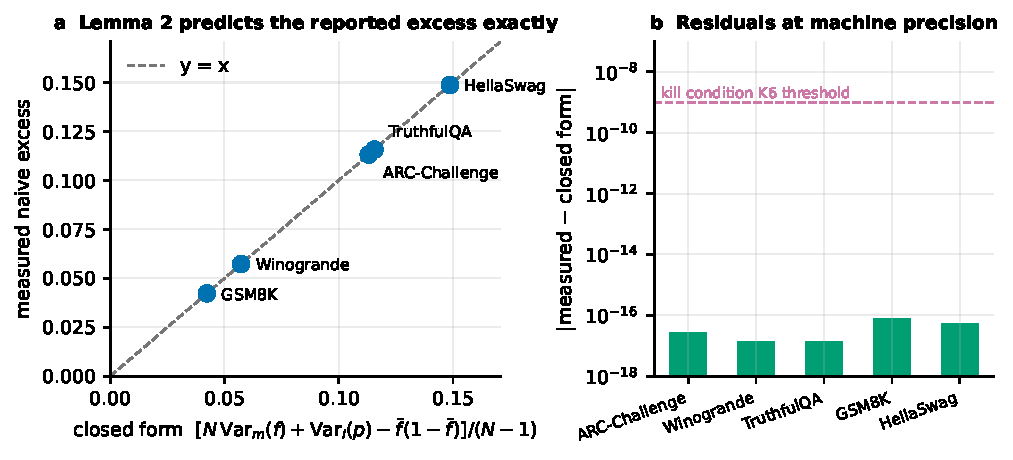
\includegraphics[width=0.92\linewidth]{../figures/fig2_closed_form.pdf}
\caption{Lemma~\ref{lem:alpha} predicts the measured excess exactly on all five benchmarks
(panel a); the residual sits at machine precision, well below the $10^{-9}$ validation
threshold set in the pre-registration (panel b).}
\label{fig:closedform}
\end{figure}

\subsection{The pre-registered dispersion statistic is refuted}

Our pre-registered primary test was whether $T=\operatorname{Var}_{i<j}(C_{ij})$ exceeds its null.
It does not do so consistently (Table~\ref{tab:T}); the pre-registered kill condition required
the effect in at least two of three primary benchmarks and it fired. We report $T$ as
uninformative rather than reinterpreting it.

\begin{table}[t]\centering\small
\begin{tabular}{lrrrr}
\toprule
Benchmark & $T$ observed & $T$ null & SES & ratio \\
\midrule
ARC-Challenge & $7.640\times10^{-3}$ & $8.331\times10^{-3}$ & $-70.9$ & $0.917$ \\
Winogrande & $1.310\times10^{-3}$ & $2.322\times10^{-3}$ & $-149.8$ & $0.564$ \\
TruthfulQA & $1.277\times10^{-2}$ & $1.164\times10^{-2}$ & $+80.1$ & $1.098$ \\
GSM8K & $4.576\times10^{-2}$ & $4.623\times10^{-2}$ & $-38.5$ & $0.990$ \\
HellaSwag & $5.098\times10^{-3}$ & $5.085\times10^{-3}$ & $+10.6$ & $1.002$ \\
\bottomrule
\end{tabular}
\caption{Independent-chain nulls, $R=200$ chains each burned in $50$ trades per model.}
\label{tab:T}
\end{table}

\subsection{What survives: effective independence}

\begin{table}[t]\centering\small
\begin{tabular}{lrrrrr}
\toprule
Benchmark & $N$ & $N_{\text{eff}}$ obs. & $N_{\text{eff}}$ null & ratio & raw (unconditioned) \\
\midrule
ARC-Challenge & 1362 & $23.6$ & $449.3\pm3.4$ & $0.052$ & $1.9$ \\
Winogrande & 1361 & $20.1$ & $493.8\pm3.0$ & $0.041$ & $3.6$ \\
TruthfulQA & 1334 & $17.4$ & $309.7\pm2.4$ & $0.056$ & $1.5$ \\
GSM8K & 1228 & $118.6$ & $553.1\pm2.2$ & $0.214$ & $2.1$ \\
HellaSwag & 1362 & $27.3$ & $958.0\pm3.2$ & $0.028$ & $1.5$ \\
\bottomrule
\end{tabular}
\caption{The last column shows why calibration is not optional: uncalibrated, the participation
ratio reads $1.5$--$3.6$, which is not a finding but the single shared difficulty eigenvalue.}
\label{tab:neff}
\end{table}

\begin{figure}[t]\centering
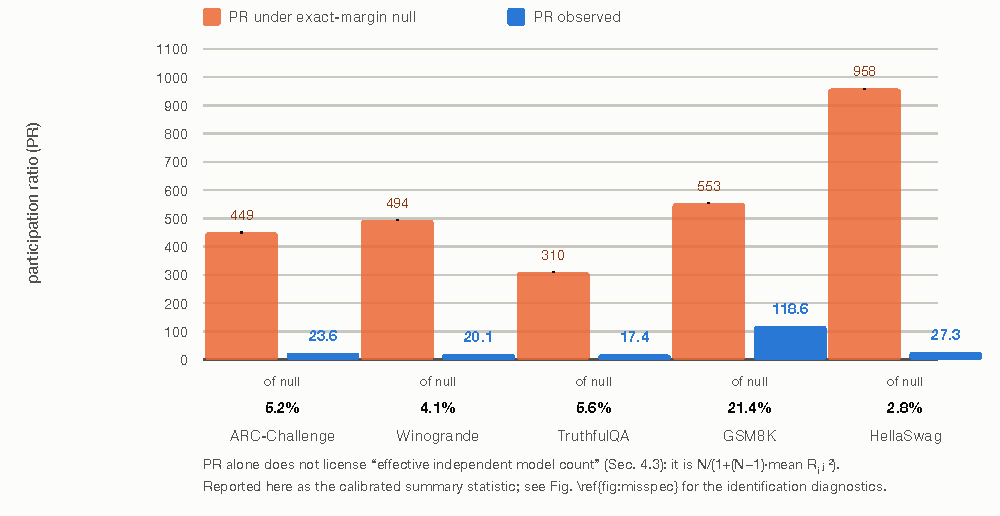
\includegraphics[width=0.92\linewidth]{../figures/fig_residual_summary.pdf}
\caption{Observed participation ratio against its exact-margin null, all five benchmarks. Read
this alongside Section~\ref{sec:notneff}: PR is reported here as a calibrated summary
statistic, not as a count of independent models.}
\label{fig:residualsummary}
\end{figure}

\subsection{Why these numbers are not an ``effective number of models''}
\label{sec:notneff}

It is tempting to read Table~\ref{tab:neff} as ``$1{,}362$ models behave like $24$''. That
reading is wrong, and the reason is algebraic. For any unit-diagonal $R$,
\[
\mathrm{PR} \;=\; \frac{(\sum_k\lambda_k)^2}{\sum_k\lambda_k^2}
\;=\; \frac{N}{1+(N-1)\,\overline{R_{ij}^2}},
\]
which we confirm to machine precision on ARC ($16.0449$ computed either way). The
eigendecomposition contributes nothing: the participation ratio is a monotone transform of the
mean squared off-diagonal residual correlation. An equicorrelated matrix --- one weak global
factor plus $N-1$ independent directions --- reproduces the reported value exactly, and so does
a partition into $24$ blocks of exact clones. The statistic cannot tell them apart, so it cannot
license a count of independent models.

The diagnostics that can tell them apart give a clear answer on ARC:
$\lambda_1^2/\sum\lambda_k^2 = 0.540$ (one-factor $\approx0.99$, clone blocks $\approx0.10$);
deflating the leading eigenvector raises PR only from $16.0$ to $46.8$, not to $\approx N$; and
five observed eigenvalues exceed the null's maximum eigenvalue of $28.7$. We therefore report
the primitive quantity, $\mathrm{rms}\,|R_{ij}| = 0.2483$ against $0.0389$ under the null, and
the count of dimensions above the null spectral edge.

\subsection{Misspecification controls: what else could produce this}

Our conditioning model is one-parameter. Any two-parameter or multidimensional structure leaves
residual signal that the margin-preserving null cannot reproduce, so we ask how much of the
effect that alone explains. Each row below is a simulated population with \emph{no} clusters, no
clones and no shared lineage --- errors conditionally independent given the item.

\begin{table}[t]\centering\small
\begin{tabular}{lrrrr}
\toprule
Generating process & PR / PR$_{\text{null}}$ & rms $|R_{ij}|$ & $\lambda_1^2/\sum\lambda^2$ & dims $>$ edge \\
\midrule
1PL, correctly specified & $1.001$ & $0.065$ & $0.105$ & 1 \\
2PL, $\mathrm{sd}(\log a)=0.35$ & $0.966$ & $0.068$ & $0.119$ & 1 \\
2PL, $\mathrm{sd}(\log a)=0.60$ & $0.862$ & $0.076$ & $0.167$ & 1 \\
two ability dimensions & $0.230$ & $0.162$ & $0.457$ & 3 \\
20 exact clone clusters & $0.112$ & $0.234$ & $0.102$ & 19 \\
\midrule
\textbf{real ARC} & $\mathbf{0.052}$ & $\mathbf{0.248}$ & $\mathbf{0.540}$ & \textbf{5} \\
\bottomrule
\end{tabular}
\caption{Discrimination heterogeneity alone cannot produce the observed effect. A
low-dimensional multi-ability structure produces much of it, and the observed spectral signature
resembles that case rather than duplicated model families.}
\label{tab:misspec}
\end{table}

\begin{figure}[t]\centering
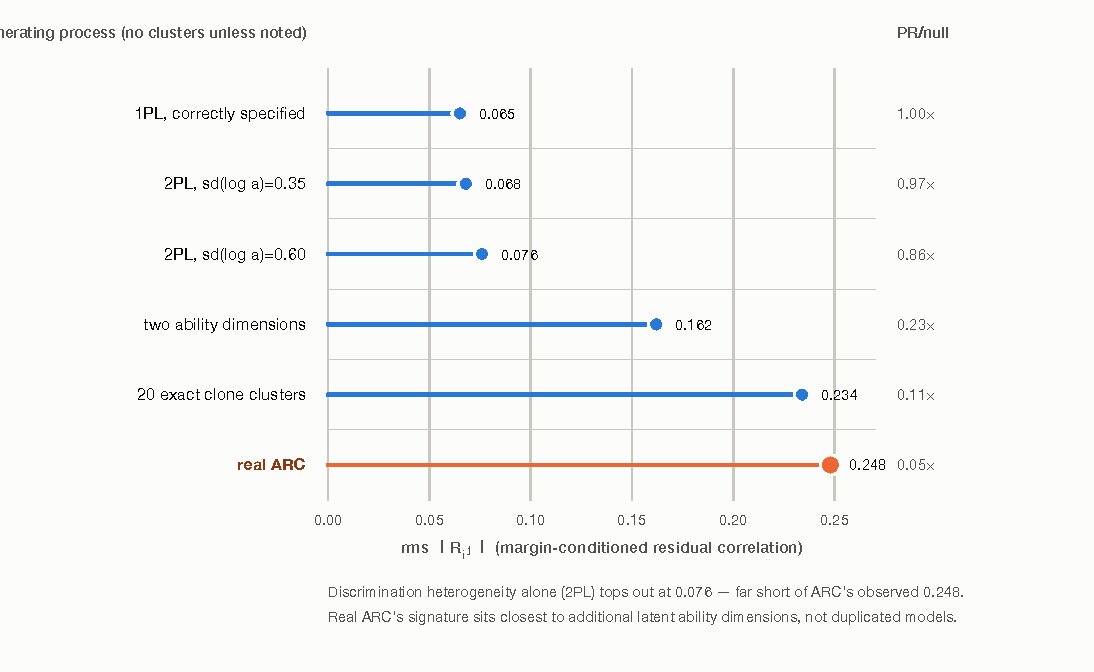
\includegraphics[width=0.92\linewidth]{../figures/fig_misspec.pdf}
\caption{Identification evidence: real ARC's residual correlation (orange) sits far beyond
what two-parameter discrimination heterogeneity alone can produce, and its
$\lambda_1^2/\sum\lambda^2$ signature (Table~\ref{tab:misspec}) matches a multi-ability
structure rather than duplicated models.}
\label{fig:misspec}
\end{figure}

Two conclusions follow. Discrimination heterogeneity is \emph{not} a sufficient explanation:
even at $\mathrm{sd}(\log a)=0.60$ it yields rms $0.076$ against the observed $0.248$. But a
small number of extra ability dimensions is a substantial one, and the observed
$\lambda_1^2/\sum\lambda^2 = 0.540$ sits near the two-dimensional case ($0.457$) and far from
the clone case ($0.102$). We therefore state the finding as: after conditioning on item
difficulty and unidimensional ability, open-model failure retains correlated structure of
roughly five dimensions and sixfold excess rms correlation, whose signature is that of
additional latent ability dimensions rather than of duplicated models.

\subsection{Reconciling two opposite-looking results}
\label{sec:reconcile}

$T$ below null and $N_{\text{eff}}$ far below null appear to conflict: since $R$ has unit
diagonal, $\operatorname{tr}R=N$ exactly and $N_{\text{eff}}=N^2/\lVert R\rVert_F^2$, so
$N_{\text{eff}}$ far below null is algebraically equivalent to the off-diagonal excess
correlations being far \emph{above} null. The resolution is exact. Because the null preserves
margins, the fitted $P$ --- and hence $E=PP^{\!\top}/M$ --- is identical for the observation and
every replicate; we measure $|\operatorname{Var}(E)_{\text{obs}}-\operatorname{Var}(E)_{\text
{null}}| = 0.000\times10^{0}$. Writing $C=E+D$,
\[
\operatorname{Var}(C)=\operatorname{Var}(E)+2\operatorname{Cov}(E,D)+\operatorname{Var}(D).
\]
On ARC: $\operatorname{Var}(D)=6.253\times10^{-4}$ against a null of $2.127\times10^{-5}$
(SES $+1613$, a $29\times$ excess), while $\operatorname{Cov}(E,D)=-6.494\times10^{-4}$ against
$-2.1\times10^{-6}$ (SES $-153$; correlation $-0.285$ versus $-0.005$). The negative covariance
outweighs the excess variance, which is exactly why $T$ reads below null. Both statistics are
correct and the arithmetic closes to the reported $\operatorname{Var}(C)$.

\begin{figure}[t]\centering
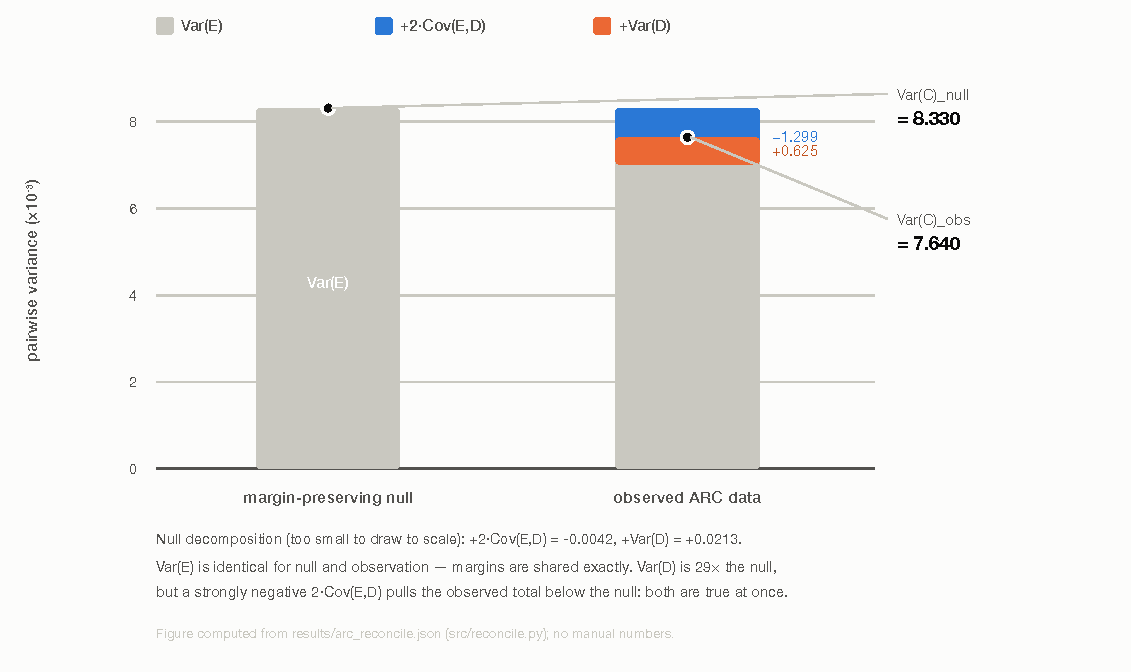
\includegraphics[width=0.92\linewidth]{../figures/fig_reconcile.pdf}
\caption{The exact decomposition $\operatorname{Var}(C)=\operatorname{Var}(E)+2
\operatorname{Cov}(E,D)+\operatorname{Var}(D)$ on ARC. $\operatorname{Var}(E)$ is identical for
null and observation by construction; the observed column's negative covariance term outweighs
its $29\times$-inflated variance term, landing below the null.}
\label{fig:reconcile}
\end{figure}

Substantively: pairs that the margin model predicts will co-fail most actually co-fail
relatively less, and vice versa. That is structured deviation from unidimensionality --- which is
what ``models cluster into a few dozen behavioural types'' means when stated in Rasch terms. We
flag that ``residual structure'' and ``Rasch misfit'' are the same observation under two
descriptions, and that our design cannot separate them.

\subsection{Robustness}
\label{sec:robust}

\paragraph{Near-duplicates.} The archive contains exact duplicates (maximum pairwise agreement
$1.0000$). Clustering models by agreement and keeping one representative per cluster: on ARC,
removing $900$ of $1{,}362$ models moves $N_{\text{eff}}$ from $23.6$ only to $29.0$; on
TruthfulQA, removing $1{,}001$ of $1{,}334$ moves it from $17.4$ to $26.2$; on GSM8K, removing
$450$ moves it from $118.6$ to $111.4$. Redundant submissions are not the mechanism.

\begin{figure}[t]\centering
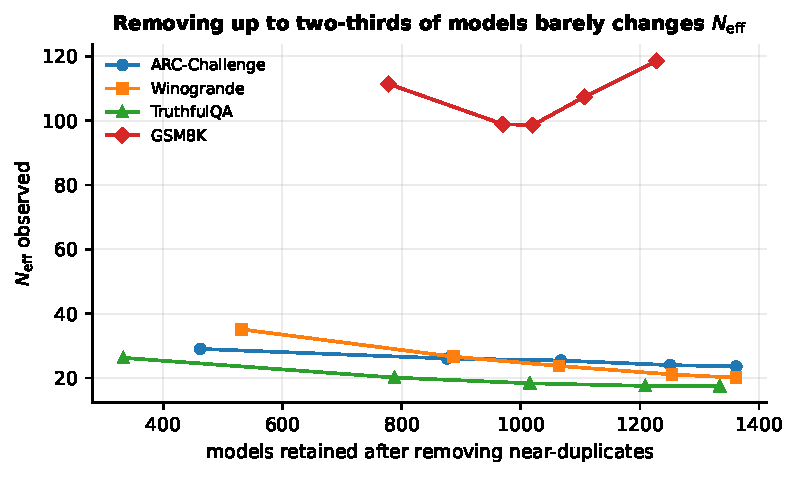
\includegraphics[width=0.92\linewidth]{../figures/fig5_dedup.pdf}
\caption{Observed participation ratio as near-duplicate models (agreement $\ge$ threshold,
one representative kept per cluster) are progressively removed. Removing up to two-thirds of
each benchmark's models moves the statistic by only a few units.}
\label{fig:dedup}
\end{figure}

\paragraph{Mixing.} $T$ plateaus by about $10$ trades per model and is flat to $200$. Independent
chains give null SD ratios $0.96$--$1.02$ versus single-chain thinning, with lag-1
autocorrelations between $-0.14$ and $+0.07$. A $2000$-trades-per-model burn-in gives an ARC
$N_{\text{eff}}$ null of $450.8$ against $449.3$ at $50$ --- a $40\times$ longer burn-in moves it
by $0.3\%$. Both margins are exactly preserved at every checkpoint.

\paragraph{Functional choice.} On ARC, $91.35\%$ of spectral mass is positive. The participation
ratio is insensitive to the treatment of negative eigenvalues: $23.6$ clipped, $23.5$ absolute,
$16.0$ raw.

\paragraph{Estimator controls.} On a matrix drawn from a Rasch margin model the dispersion
estimator reports SES $+0.05$; on eight latent model families $+6.75$; on exact clones $+2.64$;
on column-shuffled real data $-1.33$.

\subsection{Real responses: the accuracy--agreement claim survives conditioning}
\label{sec:h4}

Everything above concerns \emph{correctness} (binary failure). Section~\ref{sec:degeneracy}'s
Proposition 3 concerns \emph{which wrong answer} two models give, and predicted --- and, in
simulation, demonstrated --- that this can look like ``more correlated errors'' purely from
per-item distractor attractiveness, with no shared behaviour at all. We pre-registered a direct
test of whether that critique undermines \citet{kim2025correlated}'s specific empirical claim,
with a kill condition (K7) stated in advance: if the accuracy--agreement slope survives margin
conditioning with confidence interval excluding zero, our critique does not apply here, and we
report their finding as robust. We reconstruct each model's chosen answer from per-choice
log-likelihoods on a $600$-model ARC subsample, recovering the gold answer from cross-model
agreement where models are correct (agreement among correct models $1.0000$ on $1{,}144/1{,}172$
items; the recovered gold reproduces each model's own reported accuracy on $99.01\%$ of cells,
which we take as validating the reconstruction rather than assuming it).

\textbf{K7 fires.} The raw slope of agreement-when-both-wrong against mean pair accuracy is
$+0.585$ ($95\%$ CI $[0.577, 0.594]$); conditioned on the composition-preserving null it is
$+0.514$ ($[0.506, 0.522]$) --- an attenuation of only $12.1\%$. The claim that more accurate
models give more similar wrong answers is not an artifact of item-level distractor composition:
it survives our conditioning almost fully. We report this as prominently as the alternative,
per the pre-registration.

Two things are true at once, and both matter. The mean-level excess vanishes:
$0.7332$ observed versus $0.7324$ expected under conditional independence
($+0.00085$), essentially zero, echoing Proposition 3's degeneracy result. But the
\emph{relationship between accuracy and agreement} is not a mean-level statistic, and it is not
absorbed by the same conditioning. Composition-based conditioning and accuracy-slope
conditioning are different operations; only the latter bears on \citeauthor{kim2025correlated}'s
claim, and it does not remove it.

\section{Related work}

\citet{kim2025correlated} measure agreement-when-both-wrong across 349 models against a uniform
baseline, conditioning on model accuracy but not item difficulty, and report that larger and more
accurate models have more correlated errors. \citet{jo2026subjectivity} show that conditioning on
item difficulty via fitted IRT attenuates such correlations substantially and sometimes reverses
their sign, and argue the inference is null-dependent and hence subjective; our contribution is
to identify a null on that ladder which requires no fitting, and to report the answer there.
Foundational framing of algorithmic monoculture and outcome homogenisation is due to
\citet{kleinberg2021monoculture} and \citet{bommasani2022homogenization}. On method, the
fixed-fixed null and curveball come from ecology
\citep{connor1979,schluter1984,gotelli2000,strona2014}; the equivalent Rasch conditional
machinery from psychometrics
\citep{rasch1960,andersen1973,besag1989,ponocny2001,verhelst2008,miller2013}; the
participation-ratio and shared-mode-removal apparatus from econophysics
\citep{laloux1999,plerou1999} and statistical genetics
\citep{cheverud2001,nyholt2004,liji2005}; and the excess-matrix construction from network
backbone extraction \citep{neal2021}.

\section{Limitations}

Claims cover the evaluated open-model ecosystem on multiple-choice-style benchmarks, not deployed
proprietary systems; the societal framing is motivation, not a measured outcome, and we make no
claim about real-world screening decisions. The models are a self-selected population of
leaderboard submissions, and \citet{jo2026subjectivity} show explicitly that such inferences are
population-dependent --- a different peer set can change them.

The central limitation is identification. Our conditioning model is unidimensional, and
Table~\ref{tab:misspec} shows that additional latent ability dimensions reproduce much of the
observed effect with no shared lineage whatsoever. We can rule out discrimination heterogeneity
as a sufficient explanation, and we can rule out duplicate models, but we cannot separate
``genuine behavioural concentration'' from ``the Rasch family is too small'' --- and on the
spectral evidence the latter is the better description. Re-conditioning on a fitted 2PL or
low-rank logistic model would sharpen this at the cost of the exactness that motivates the
design; that trade-off is the natural next step.

We also report a negative methodological result about our own pre-registered plan: the
participation ratio does not measure an effective number of independent models
(Section~\ref{sec:notneff}), and we have removed that interpretation rather than retain it.

Pre-registered kill condition K5 failed --- declared \texttt{base\_model} coverage was $23.3\%$
against a $40\%$ threshold, with $315$ of $1{,}362$ model repositories no longer retrievable ---
so the lineage decomposition is dropped rather than estimated on a biased subset.

Section~\ref{sec:h4}'s real-response result is a limitation on the paper's own critique, stated
plainly: Proposition 3 shows composition alone \emph{can} manufacture apparent agreement, but on
real ARC responses the specific published claim it was aimed at does not turn out to be an
instance of that artifact. The two findings do not contradict --- they concern different
statistics, mean-level agreement versus the accuracy--agreement slope --- but a reader taking
only the abstract's mention of Proposition 3 could reasonably expect more debunking than the
data supports, which is why the full result is reported in Section~\ref{sec:h4} rather than
folded silently into the mean-level finding.

\section{Reproducibility and use of AI assistance}

All code, the harmonised substrate, and every results artifact are released; each number traces
to a JSON file emitted by an executed run, and the propositions are asserted as unit tests. The
study was pre-registered before the confirmatory analysis, with two dated amendments recorded
before any confirmatory statistic was computed; one pre-registered hypothesis was refuted by its
own kill condition and is reported as refuted.

This work used a large language model (Claude, Anthropic) as a coding and analysis assistant: it
wrote the harvesting, estimation and figure code and assisted in drafting and in the adversarial
prior-art review that led to Section~\ref{sec:degeneracy} being rewritten from claimed novelty to
attribution. The author directed the research, specified and pre-registered the hypotheses and
kill conditions, verified the derivations, and takes full responsibility for the content, in line
with COPE guidance that AI tools cannot be authors.

\bibliographystyle{plainnat}
\begin{thebibliography}{99}
\small
\bibitem[Andersen(1973)]{andersen1973} E.~B. Andersen. A goodness of fit test for the Rasch model. \emph{Psychometrika}, 38:123--140, 1973.
\bibitem[Besag \& Clifford(1989)]{besag1989} J.~Besag and P.~Clifford. Generalized Monte Carlo significance tests. \emph{Biometrika}, 76:633--642, 1989.
\bibitem[Bommasani et al.(2022)]{bommasani2022homogenization} R.~Bommasani, K.~A. Creel, A.~Kumar, D.~Jurafsky, and P.~Liang. Picking on the same person: Does algorithmic monoculture homogenize outcomes? \emph{NeurIPS}, 2022.
\bibitem[Cheverud(2001)]{cheverud2001} J.~M. Cheverud. A simple correction for multiple comparisons in interval mapping genome scans. \emph{Heredity}, 87:52--58, 2001.
\bibitem[Connor \& Simberloff(1979)]{connor1979} E.~F. Connor and D.~Simberloff. The assembly of species communities: chance or competition? \emph{Ecology}, 60:1132--1140, 1979.
\bibitem[Cronbach(1951)]{cronbach1951} L.~J. Cronbach. Coefficient alpha and the internal structure of tests. \emph{Psychometrika}, 16:297--334, 1951.
\bibitem[Fleiss(1971)]{fleiss1971} J.~L. Fleiss. Measuring nominal scale agreement among many raters. \emph{Psychological Bulletin}, 76:378--382, 1971.
\bibitem[Gotelli(2000)]{gotelli2000} N.~J. Gotelli. Null model analysis of species co-occurrence patterns. \emph{Ecology}, 81(9):2606--2621, 2000.
\bibitem[Gotelli \& Ulrich(2012)]{gotelliulrich2012} N.~J. Gotelli and W.~Ulrich. Statistical challenges in null model analysis. \emph{Oikos}, 121:171--180, 2012.
\bibitem[Jo et al.(2026)]{jo2026subjectivity} N.~Jo, N.~Garg, and M.~Raghavan. The subjectivity of monoculture. \emph{arXiv:2602.24086}, 2026.
\bibitem[Kim et al.(2025)]{kim2025correlated} Correlated errors in large language models. \emph{arXiv:2506.07962}, 2025.
\bibitem[Kleinberg \& Raghavan(2021)]{kleinberg2021monoculture} J.~Kleinberg and M.~Raghavan. Algorithmic monoculture and social welfare. \emph{PNAS}, 118(22), 2021.
\bibitem[Kuder \& Richardson(1937)]{kuder1937} G.~F. Kuder and M.~W. Richardson. The theory of the estimation of test reliability. \emph{Psychometrika}, 2:151--160, 1937.
\bibitem[Laloux et al.(1999)]{laloux1999} L.~Laloux, P.~Cizeau, J.-P. Bouchaud, and M.~Potters. Noise dressing of financial correlation matrices. \emph{Physical Review Letters}, 83:1467, 1999.
\bibitem[Li \& Ji(2005)]{liji2005} J.~Li and L.~Ji. Adjusting multiple testing in multilocus analyses using the eigenvalues of a correlation matrix. \emph{Heredity}, 95:221--227, 2005.
\bibitem[Linacre(1998)]{linacre1998} J.~M. Linacre. Structure in Rasch residuals: why principal components analysis? \emph{Rasch Measurement Transactions}, 12:636, 1998.
\bibitem[Miller \& Harrison(2013)]{miller2013} J.~W. Miller and M.~T. Harrison. Exact sampling and counting for fixed-margin matrices. \emph{Annals of Statistics}, 41:1569--1592, 2013.
\bibitem[Neal et al.(2021)]{neal2021} Z.~P. Neal, R.~Domagalski, and B.~Sagan. Comparing alternatives to the fixed degree sequence model for extracting the backbone of bipartite projections. \emph{Scientific Reports}, 11:23929, 2021.
\bibitem[Nyholt(2004)]{nyholt2004} D.~R. Nyholt. A simple correction for multiple testing for single-nucleotide polymorphisms in linkage disequilibrium with each other. \emph{American Journal of Human Genetics}, 74:765--769, 2004.
\bibitem[Plerou et al.(1999)]{plerou1999} V.~Plerou, P.~Gopikrishnan, B.~Rosenow, L.~A.~N. Amaral, and H.~E. Stanley. Universal and nonuniversal properties of cross correlations in financial time series. \emph{Physical Review Letters}, 83:1471, 1999.
\bibitem[Ponocny(2001)]{ponocny2001} I.~Ponocny. Nonparametric goodness-of-fit tests for the Rasch model. \emph{Psychometrika}, 66:437--460, 2001.
\bibitem[Rasch(1960)]{rasch1960} G.~Rasch. \emph{Probabilistic Models for Some Intelligence and Attainment Tests}. Danmarks P\ae dagogiske Institut, 1960.
\bibitem[Schluter(1984)]{schluter1984} D.~Schluter. A variance test for detecting species associations, with some example applications. \emph{Ecology}, 65:998--1005, 1984.
\bibitem[Strona et al.(2014)]{strona2014} G.~Strona, D.~Nappo, F.~Boccacci, S.~Fattorini, and J.~San-Miguel-Ayanz. A fast and unbiased procedure to randomize ecological binary matrices with fixed row and column totals. \emph{Nature Communications}, 5:4114, 2014.
\bibitem[van der Linden \& Sotaridona(2006)]{vanderlinden2006} W.~J. van der Linden and L.~Sotaridona. Detecting answer copying when the regular response process follows a known response model. \emph{Journal of Educational and Behavioral Statistics}, 31:283--304, 2006.
\bibitem[Verhelst(2008)]{verhelst2008} N.~D. Verhelst. An efficient MCMC algorithm to sample binary matrices with fixed marginals. \emph{Psychometrika}, 73:705--728, 2008.
\bibitem[Wollack(1997)]{wollack1997} J.~A. Wollack. A nominal response model approach for detecting answer copying. \emph{Applied Psychological Measurement}, 21:307--320, 1997.
\bibitem[Yule(1903)]{yule1903} G.~U. Yule. Notes on the theory of association of attributes in statistics. \emph{Biometrika}, 2:121--134, 1903.
\end{thebibliography}

\end{document}
